\chapter{Framework web}

\section{Motivations}
\textit{Construction d'un framework d'interface web sur la base des signaux introduits précédemment.}

\textit{Développement spécifiquement pour Scala.js. Il existe de nombreux bindings par exemple pour React ou Angular en Scala.js, mais l'utilisation d'un framework conçu pour JavaScript en Scala.js n'est pas toujours l'expérience la plus agréable. Volonté de disposer d'une API conçue pour le langage Scala.}

\section{Spécifications} \label{sec:web-specs}

\textit{L'architecture du framework web est encore à un stade très primitif.}

\subsection{Composant}
\textit{Définition de nouveau composant. Un composant est défini par:}
\begin{itemize}
	\item \emph{Un sélecteur}: correspondant à la balise HTML qui sera définie pour ce composant. Ce nom doit comporter un tiret (selon la spécification \emph{Custom Elements}).
	\item \emph{Un template}: une structure HTML pouvant contenir des expressions de data-binding avec des données réactives sous la forme de signaux
	\item \emph{Une feuille de styles}: pouvant être utilisée pour définir l'apparence visuelle du composant
	\item \emph{Un behavior}: comportement de l'élément en réponses aux interactions. Implémentées en tant que classe Scala.js.
\end{itemize}

\subsection{Template}
\textit{Défini à partir de code HTML, il est parsé et compilé par le framework en un objet de type \texttt{Template} qui est alors utilisé pour chaque instance du composant.}

\textit{L'opération de compilation ne s'effectue qu'une seule fois à la première utilisation du composant puis réutilisé. La forme compilée et optimisée pour la création de nombreuses instances du template.}

\textit{Il y a donc un coût important lors de la première utilisation puis un coût minimal lors des utilisations futures, ce qui est cohérent avec l'utilisation des objets templates: définis une fois par composant, instantiés de nombreuses fois.}

\textit{Le template peut contenir des expressions de data-bindings qui seront utilisée pour y inclure dynamiquement des données provenant de signaux réactif.}

\subsection{Expressions}
\textit{La syntaxe des expressions est fortement inspirée des expressions de Angular 2, sémantiquement adaptée pour correspondre à une usage combiné aux signaux.}

\textit{Parser construit avec les "Parser Combinators" de Scala. Production d'un AST représentant l'expression puis optimisation de cet arbre.}

\textit{De façon similaire aux templates: coût initial important puis faible coût lors de l'utilisation.}

\textit{L'AST est passé à un interpréteur en même temps qu'une contexte d'évaluation spécifiant les variables globales à disposition est le composant dans lequel l'expression s'exécute.}

\textit{Peut être une section à part entière}

\subsection{Feuille de styles}
\textit{Simple morceau de code CSS qui sera injecté dans le sous-arbre Shadow DOM correspondant au composant.}

\subsection{Behavior}
\textit{Définition d'une classe Scala qui étend \texttt{XuenBehavior}, qui étend lui même l'interface DOM \texttt{HTMLElement}.}
\section{Solutions existantes}
\section{Implémentation}

\subsection{Vue d'ensemble}
\begin{figure}[h]
	\centering
	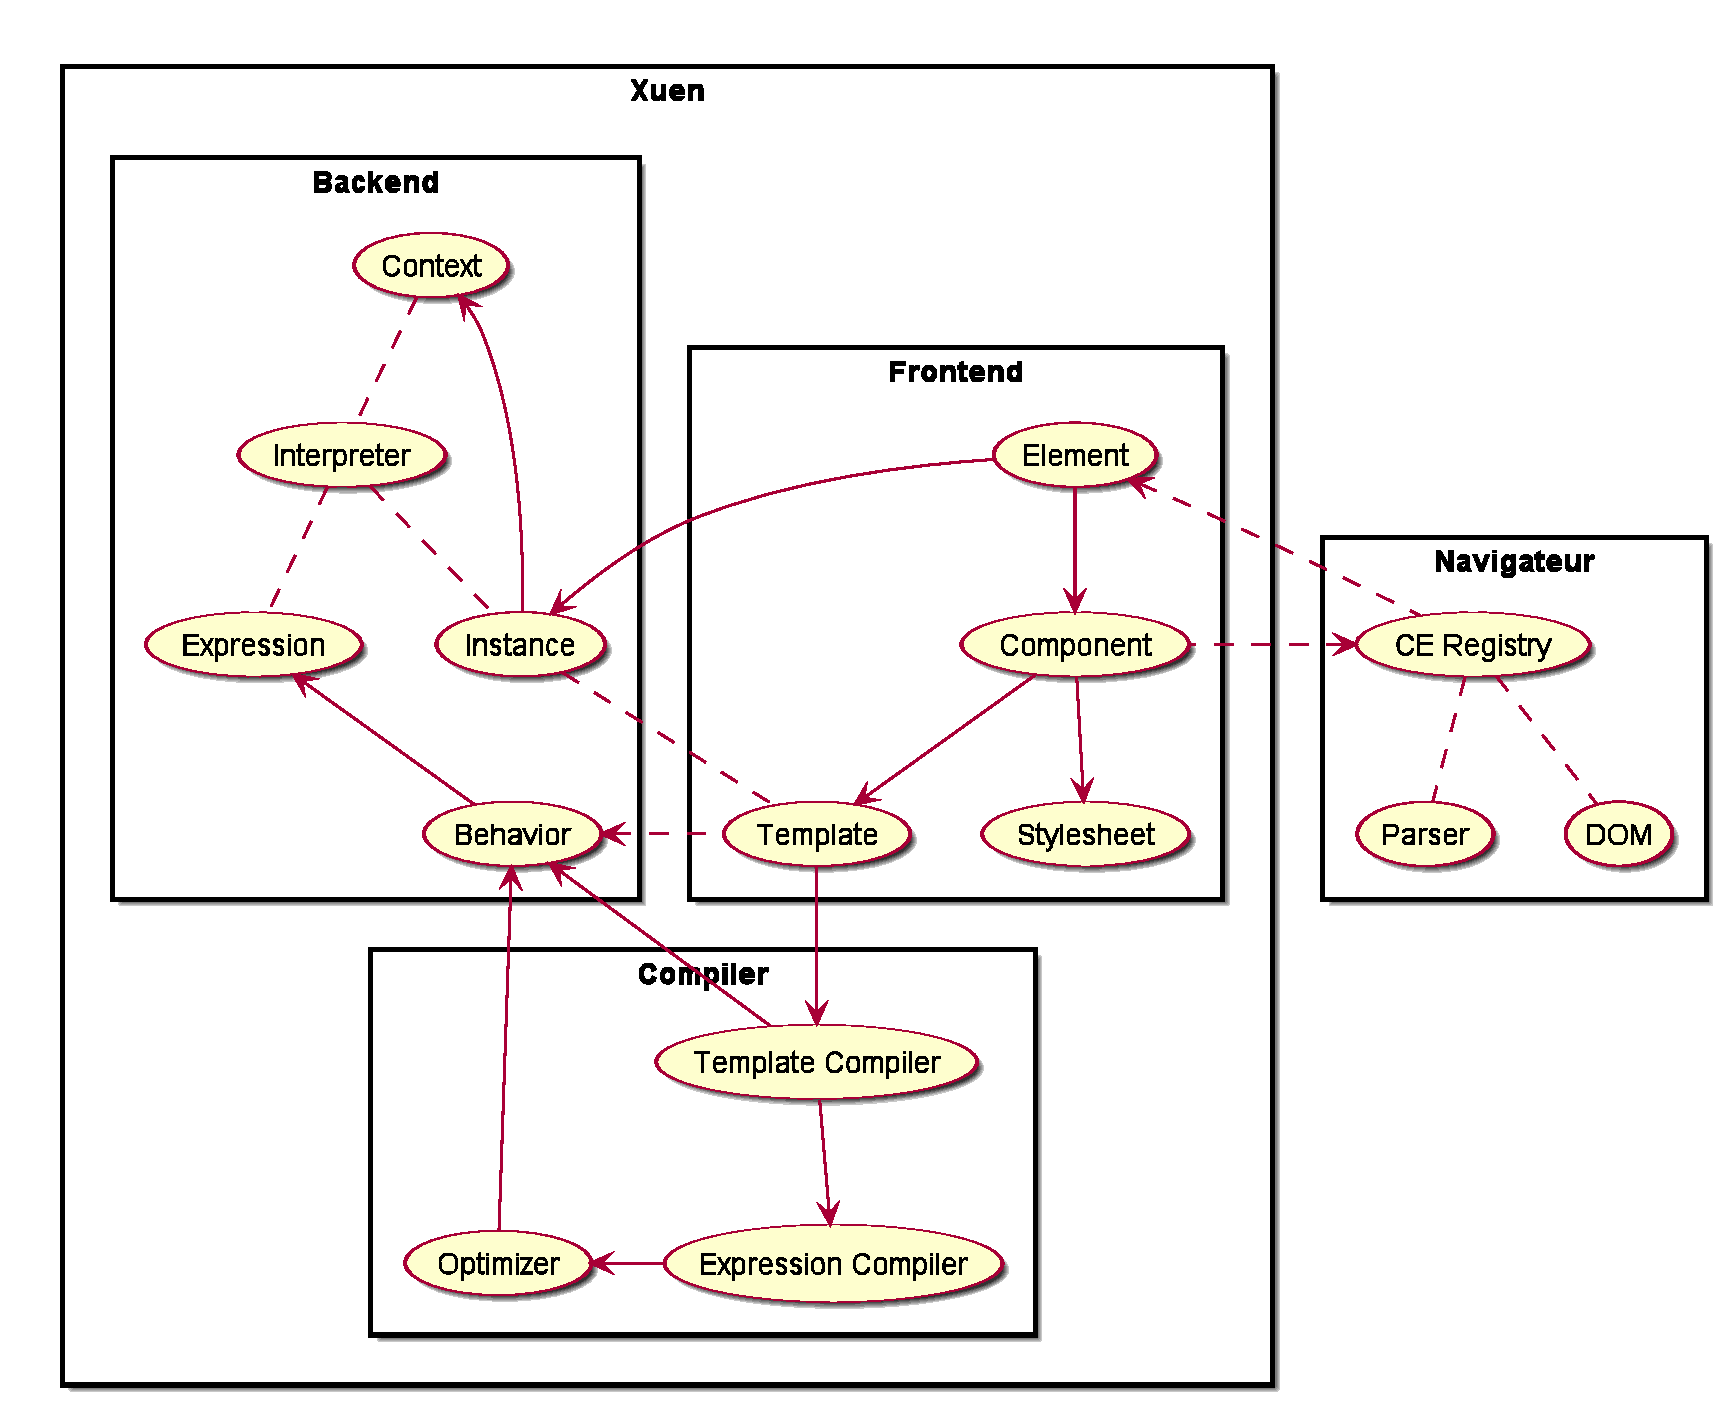
\includegraphics[width=\textwidth]{img/web_overview.eps}
	\caption{Vue d'ensemble de l'implémentation du framework Web}
	\label{fig:web-overview}
\end{figure}

L'implémentation du framework web de Xuen peut être décomposé en 3 grandes parties, tel qu'illustré par la figure \ref{fig:web-overview}.

\begin{enumerate}
	\item La partie \emph{front-end} est exposée directement au développeur. Elle est utilisée pour déclarer les composants personnalisés de l'application, leurs comportement et structure.
	\item La partie \emph{back-end} est utilisée par le framework lorsqu'un élément est instancié dans le document. Elle fournit les outils nécessaires à l'implémentation des comportements dynamiques du template de cet élément et l'interface avec le système de signaux par le biais des expressions.
	\item Finalement le système de compilation est utilisé lors de la définition d'un nouveau composant pour transformer le code source HTML du template en une instance de la classe \texttt{Template}, encapsulant à la fois une structure pré-traitée du template, des modèles pour construire les comportements dynamiques de ce template et des expressions sous forme d'arbres syntaxiques prêts à être interprétés.  
\end{enumerate}

L'objectif de la partie de compilation est de réduire l'impact du traitement du template au \emph{runtime}. En effet, l'instanciation d'un template se base sur les outils fournis par le navigateur, notamment le parser HTML et son implémentation du DOM afin parcourir et traiter la structure fournie sous forme de code HTML.

En compilant le template et les expressions dès la déclaration, il n'est plus nécessaire de le faire lors de l'instanciation, ce qui permet un investissement fixe au chargement de l'application et des performances accrues lors de son fonctionnement.

Cette structure est en grande partie reprise d'un projet personnel antérieur. La plupart des éléments ont été repensés et réimplémentés, principalement pour les adapter au nouveaux standards \emph{Web Components} version \emph{v1} (par opposition à la version antérieure \emph{v0}). Le parser d'expression a quant à lui été réécrit, passant d'une implémentation fortement inspirée du parser d'expression du framework Angular 2, mais en Scala, à une version développée avec la bibliothèque \emph{scala-parser-combinators} \cite{scala-parser-combinators}, plus propre et idiomatique. La grammaire du langage n'a cependant pas été significativement modifiée. L'optimisateur d'expressions est réutilisé pratiquement tel quel.

\subsection{Processus de compilation du template}

Le template est fourni à la bibliothèque sous forme de code source HTML. La première opération consiste donc à construire dynamiquement un élément \texttt{<template>} et à y insérer le code du développeur. Le parser HTML du navigateur sera alors invoqué pour construire une structure de nœuds DOM. Cette structure est ensuite parcourue de façon récursive en commençant à l'élément template créé précédemment.

\begin{itemize}
	\item Premièrement, la nature du noeud en cours est déterminée. S'il s'agit d'un nœud \texttt{Text} ou \texttt{Comment}, son contenu est scanné pour y identifier d'éventuelles interpolations.
	\item Si le nœud est un élément, ses attributs sont observés.
	\item Si l'élément est annoté d'une transformation \texttt{*if} ou \texttt{*for}, cette transformation est appliquée.
	\item Si l'élément possède des annotations de \emph{data-binding}, celles-ci sont traitées.
	\item Les valeurs des attributs restants qui ne sont ni des transformations ni des annotations de \emph{data-binding} sont scannées pour y identifier des interpolations.
	\item Une fois l'élément lui-même entièrement traité, l'ensemble de ses enfants est parcouru, réitérant le processus.
\end{itemize}

Pour chaque nœud DOM devant être associé à un comportement dynamique, un \texttt{Behavior} est créé. Celui-ci est identifié par un numéro incrémenté à chaque nouvelle instance. Il sera de modèle pour la construction du comportement dynamique en question. Tous les \texttt{Behavior}s créés pour un template son rassemblé dans une \texttt{Map} contenue dans l'objet \texttt{Template} resultant. L'élément auquel le comportement doit être attaché est quant à lui décoré d'un attribut \texttt{xuen:behavior="..."} indiquant l'identifiant du comportement associé à ce nœud.

Si l'élément ne peut pas posséder d'attribut, c'est à dire lorsqu'il s'agit d'un nœud \texttt{Text} ou \texttt{Comment}, un élément \emph{placeholder} \texttt{<xuen:placeholder>} est inséré à sa place dans l'arbre DOM du template et l'attribut est placé sur cet élément. Dans ce cas, lors de la construction du comportement au moment de l'instanciation du template, l'élément \emph{placeholder} sera en premier lieu remplacé par un nœud correspondant à l'original puis le comportement spécifique de ce nœud sera implémenté.

Un \texttt{Behavior} peut en réalité implémenter plus d'un comportement pour un même élément. Si deux annotations sont présentes sur un même élément, le \texttt{Behavior} construit à l'occasion du traitement de la première annotation est réutilisé pour la deuxième annotation. L'objet \texttt{Behavior} sera donc en charge de construire deux comportements dynamiques différents sur le même élément.

À l'inverse de la compilation, le processus d'instanciation est relativement simple. Le template est à présent sous forme normalisée, tous les comportements sont attachés à des éléments annotés par l'attribut \texttt{xuen:behavior}. Juste avant d'implémenter les comportements dynamiques, l'objet template est cloné pour construire une nouvelle structure indépendante de l'originale qui est conservée en tant que modèle. La bibliothèque utilise alors la \texttt{Map} associant les identifiants des différents comportements enregistrés avec les objets \texttt{Behavior} encapsulant la logique de construction pour instancier à proprement parler ces comportements.

Le sélecteur CSS \texttt{[xuen:behavior="..."]} est utilisé pour récupérer l'élément sur lequel le comportement doit être appliqué puis la méthode \texttt{build} de l'objet \texttt{Behavior} est invoquée avec la référence vers l'élément courant. Cette méthode va alors instancier à proprement l'ensemble des comportements liés à cet élément.

De façon générale \emph{instancier un comportement} implique construire une paire (signal, observateur) qui implémentera le comportement désiré. Cette paire est initialement construite déconnectée. Une fois l'élément hôte connecté, son template est \emph{activé} ce qui entraine la liaison  des observateurs avec le signal associé et donc la mise en place du comportement dynamique.

Lorsqu'un élément est déconnecté, son template est \emph{désactivé}. Cette opération déconnecte l'ensemble des signaux et observateurs utilisé dans l'implémentation de ce template, assurant ainsi qu'il n'existe plus de lien entre le reste du système et l'élément déconnecté. Sans cette étape, il existe un risque que les éléments ne puissent pas être désalloués par le \emph{garbage collector} puisqu'une référence subsiste entre le reste du graphe de signaux et eux.

\subsection{Ordre de construction des \emph{Custom Elements}}

La spécifique \emph{Custom Elements} \cite{w3c-custom-elements} défini très précisément la façon dont un élément personnalisé est initialisé par le navigateur. Cette procédure, appelée \emph{upgrade} \cite[\small 2.5 Upgrades]{w3c-custom-elements}, implique une combinaison de piles et de queues pour enregistrer les actions à effectuer par le navigateur au fil de l'analyse du document HTML.

De plus la notion de \emph{connexion} au document est introduite: un élément est \emph{connecté} si il fait partie de la hiérarchie du document, \emph{déconnecté} s'il s'agit d'un élément flottant hors de l'arbre DOM principal.

L'\emph{upgrade} d'un élément ne s'effectue en principe que si cet élément est \emph{connecté} au document. Sauf s'il s'agit d'un élément étant explicitement créé par l'utilisateur. Ainsi l'utilisation de la méthode \texttt{createElement} avec un élément personnalisé provoque l'\emph{upgrade} instantané de l'élément créé, mais laisse les éléments de son template dans l'état non-\emph{upgradé}, car ceux-ci n'ont pas été instancié explicitement et que leur parent, en l'occurrence l'élément créé par \texttt{createElement}, n'est pas encore inséré dans le document; ils ne sont donc pas considérés \emph{connectés}.

Le constructeur de l'élément racine est donc invoqué alors que le constructeur de ses enfants n'a pas encore été invoqué. Hors, il est déjà possible d'utiliser \texttt{querySelector} pour accéder à ces éléments non-initialisés.

Le problème s'amplifie lorsque l'élément parent devient \emph{connecté}. Le mécanisme de queues décrit dans le standard implique que l'appel du \emph{callback} de l'élément parent est planifié avant la considération des éléments enfants. Par conséquent, la méthode \texttt{connecteCallback} est invoquée sur l'élément parent, une fois encore, avant que ses enfants n'aient eu l'occasion de s'initialiser.

Dans Xuen, le \emph{callback} de connexion est utilisé pour activer le template de l'élément parent, construisant alors l'ensemble des liens de \emph{data-binding} entre parent et enfants. Si un élément enfant n'est pas encore instancié à ce moment là, les points de connexion sous forme de signaux permettant le \emph{data-binding} ne sont pas encore disponibles et le système est alors laissé dans un état totalement inutilisable.

Afin de contourner ce problème, l'initialisation d'un élément personnalisé place temporairement les éléments de son template dans l'élément \texttt{<body>} du document, forçant ainsi l'\emph{upgrade} de ses éléments enfants. Ces éléments sont par la suite déplacés dans le \emph{Shadow DOM} de l'élément, cette fois-ci dans l'état initialisé. Cette opération s'effectue dans le constructeur de la classe \texttt{Element} du framework, avant le constructeur de la sous-classe implémentée par le développeur. Celui-ci est donc libre d'accéder aux éléments du template du composant avec la garantie que ceux-ci seront initialisés.

Cette sémantique imposée par le standard est déroutante. Le fait de retarder l'\emph{upgrade} d'un élément à sa connexion est déjà étonnant, mais appeler le \emph{callback} de connexion de son parent avant de considérer l'\emph{upgrade} des enfants est réellement problématique.

Le standard conseille de retarder les opérations d'initialisation à la première invocation du \emph{callback} de connexion. Par conséquent, accéder aux éléments enfants lors de l'invocation du constructeur peut sembler être une mauvaise pratique. En revanche, il n'est pas cohérent que ces éléments ne soient toujours pas initialisés au moment où l'élément parent devient connecté. Comment le développeur est-il sensé configurer les composants de son template si ceux-ci ne sont pas encore entièrement construits ?
